% ---------------------------------------------------------
% Template LaTeX para a Revista Contemporânea
% Configurado para XeLaTeX (Uso da fonte Verdana)
% ---------------------------------------------------------
\documentclass[12pt,a4paper]{article}

% --- Pacotes de Idioma e Codificação ---
\usepackage{polyglossia}
\setmainlanguage{portuguese}
\setotherlanguages{english,spanish}

% --- Pacotes de Fontes (Requer XeLaTeX/LuaLaTeX) ---
\usepackage{fontspec}
\setmainfont{Verdana}

% --- Pacotes de Formatação de Texto ---
\usepackage[top=3cm, left=3cm, right=2cm, bottom=2cm]{geometry}
\usepackage{setspace}
\onehalfspacing % Espaçamento 1.5 no corpo do texto

% --- Pacotes de Elementos Gráficos e Tabelas ---
\usepackage{graphicx}
\usepackage{booktabs}
\usepackage{caption}
\usepackage{float}

% --- Configuração de Legendas (Captions) ---
% Verdana 10, Espaçamento simples, Título ACIMA, Fonte ABAIXO
\DeclareCaptionFont{tenpt}{\fontsize{10}{12}\selectfont}
\captionsetup{
    font={tenpt, bf},
    labelfont={tenpt, bf},
    labelsep=period,
    justification=centering,
    singlelinecheck=false,
    skip=10pt
}
\newcommand{\source}[1]{
    \begin{center}
        \fontsize{10}{12}\selectfont Fonte: #1
    \end{center}
}

% --- Pacotes Matemáticos ---
\usepackage{amsmath}
\usepackage{amsfonts}
\usepackage{amssymb}

% --- Pacote de Citações (ABNT) ---
\usepackage[style=abnt, backend=biber]{biblatex}

% --- Configuração de Títulos (Headings) ---
\usepackage{titlesec}

% Nível 1: Introdução (Negrito, Verdana 12, Primeira letra Maiúscula)
\titleformat{\section}
  {\normalfont\large\bfseries}{\thesection.}{0.5em}{}
% Nível 2: 1.1 Referencial Teórico (Não Negrito, Verdana 12)
\titleformat{\subsection}
  {\normalfont\large}{\thesubsection}{0.5em}{}
% Nível 3: 1.1.1 Definição (Negrito)
\titleformat{\subsubsection}
  {\normalfont\normalsize\bfseries}{\thesubsubsection}{0.5em}{}

% --- Comandos Customizados ---

% Metadados do Jornal
\newcommand{\journalheader}{
    \noindent \textbf{Contemporânea} \\
    \textit{Contemporary Journal} \\
    Vol.X No.X: 01-xx, 202X \\
    ISSN: 2447-0961 \\
    \textbf{Artigo}
}

% Títulos em 3 línguas
\newcommand{\articletitles}[3]{
    \begin{center}
        \fontsize{14}{16}\selectfont \textbf{#1} \\ \vspace{0.3cm}
        \fontsize{12}{14}\selectfont #2 \\ \vspace{0.3cm}
        \fontsize{12}{14}\selectfont #3
    \end{center}
}

% Bloco de Autor
\newcommand{\authorinfo}[5]{
    \noindent \textbf{#1} \\
    #2 \\
    Instituição de formação: #3 \\
    Endereço: #4 \\
    E-mail: #5 \\ \vspace{0.5cm}
}

% Bloco de Resumo (Espaçamento Simples)
\newenvironment{abstractblock}[2]{
    \begin{singlespace}
    \noindent \textbf{#1:} #2
    \end{singlespace}
}

% ---------------------------------------------------------


\addbibresource{../../referencias.bib}

\begin{document}

\journalheader

\vspace{1cm}

\articletitles{SISTEMAS DE RECOMENDAÇÃO E SOBERANIA ATENCIONAL: O MODELO BE-PRODUCTIVE COMO ARQUITETURA DE MITIGAÇÃO DA SOBRECARGA COGNITIVA NO CAPITALISMO DE VIGILÂNCIA}{RECOMMENDATION SYSTEMS AND ATTENTIONAL SOVEREIGNTY: THE BE-PRODUCTIVE MODEL AS AN ARCHITECTURE TO MITIGATE COGNITIVE OVERLOAD IN SURVEILLANCE CAPITALISM}{SISTEMAS DE RECOMENDACIÓN Y SOBERANÍA ATENCIONAL: EL MODELO BE-PRODUCTIVE COMO ARQUITECTURA DE MITIGACIÓN DE LA SOBRECARGA COGNITIVA EN EL CAPITALISMO DE VIGILANCIA}

\vspace{0.5cm}

\noindent DOI: 10.56083/RCVXNX- \\
Receipt of originals: 02/04/2024 \\
Acceptance for publication: 02/23/2024

\vspace{0.5cm}

\authorinfo{Fellype Samuel Melo}{Graduando em Análise e Desenvolvimento de Sistemas}{FAETERJ-Rio}{Rio de Janeiro, RJ, Brasil}{fellype.24104708360042@faeterj-rio.edu.br}

\authorinfo{Felipe Farias}{Graduando em Análise e Desenvolvimento de Sistemas}{FAETERJ-Rio}{Rio de Janeiro, RJ, Brasil}{felipe.23204708360023@faeterj-rio.edu.br}

\authorinfo{Ricardo Marciano}{Doutor em História das Ciências e Pós-Doutorando (FIOCRUZ)}{FAETERJ-Rio / FIOCRUZ}{Rio de Janeiro, RJ, Brasil}{ricardo.marciano@faeterj-rio.edu.br}

\vspace{0.5cm}

\begin{abstractblock}{RESUMO}{No paradigma do capitalismo de vigilância, os sistemas de recomendação operam primordialmente para a maximização do engajamento de curto prazo, negligenciando os custos cognitivos impostos ao usuário. Essa dinâmica frequentemente resulta em fadiga atencional e sequestro da agência deliberativa. O presente artigo propõe e valida o modelo \textit{Be-Productive}, uma arquitetura algorítmica desenhada para priorizar a soberania atencional e a utilidade persistente através de curadoria intencional. A proposta integra a modelagem de Processos de Hawkes para decompor regimes de consumo e uma Equação Diferencial Ordinária (EDO) para monitoramento local da reserva cognitiva via \textit{Edge AI}. A validação foi conduzida por Simulação Baseada em Agentes (ABM) com mil indivíduos simulados. A implementação demonstrou robustez na preservação da reserva cognitiva (Cohen’s $d = 3,25$; $p < 10^{-300}$) e redução da divergência entre a intenção declarada e o consumo efetivo. Os achados indicam a viabilidade técnica de sistemas \textit{Value-Aligned} que reconciliam eficiência algorítmica com a integridade psicológica dos usuários.}
\end{abstractblock}
\noindent \textbf{PALAVRAS-CHAVE:} Sistemas de Recomendação, Capitalismo de Vigilância, Sobrecarga Cognitiva, Processos de Hawkes, Ética Algorítmica.

\vspace{0.3cm}

\begin{abstractblock}{ABSTRACT}{Within the paradigm of surveillance capitalism, recommendation systems primarily function to maximize short-term engagement, often disregarding the cognitive costs imposed on users. This dynamic frequently leads to attentional fatigue and the hijacking of deliberative agency. This paper proposes and validates the \textit{Be-Productive} model, an algorithmic architecture designed to prioritize attentional sovereignty and persistent utility through intentional curation. The proposal integrates Hawkes Processes modeling to decompose consumption regimes and an Ordinary Differential Equation (ODE) for local monitoring of cognitive reserve via Edge AI. Validation was conducted through Agent-Based Modeling (ABM) with a thousand simulated individuals. The implementation showed robustness in preserving cognitive reserve (Cohen’s $d = 3.25$; $p < 10^{-300}$) and reducing the divergence between declared intention and actual consumption. Findings indicate the technical feasibility of Value-Aligned systems that reconcile algorithmic efficiency with users' psychological integrity.}
\end{abstractblock}
\noindent \textbf{KEYWORDS:} Recommendation Systems, Surveillance Capitalism, Cognitive Overload, Hawkes Processes, Algorithmic Ethics.

\vspace{0.3cm}

\begin{abstractblock}{RESUMEN}{En el paradigma del capitalismo de vigilancia, los sistemas de recomendación operan primordialmente para maximizar el compromiso a corto plazo, descuidando los costos cognitivos impuestos al usuario. Esta dinámica suele derivar en fatiga atencional y el secuestro de la agencia deliberativa. Este artículo propone y valida el modelo \textit{Be-Productive}, una arquitectura algorítmica diseñada para priorizar la soberanía atencional y la utilidad persistente mediante la curaduría intencional. La propuesta integra el modelado de Procesos de Hawkes para descomponer regímenes de consumo y una Ecuación Diferencial Ordinaria (EDO) para el monitoreo local de la reserva cognitiva mediante \textit{Edge AI}. La validación se realizó a través de Simulación Basada en Agentes (ABM) con mil individuos simulados. La implementación demostró solidez en la preservación de la reserva cognitiva (Cohen’s $d = 3,25$; $p < 10^{-300}$) y reducción de la divergencia entre la intención declarada y el consumo efectivo. Los hallazgos indican la viabilidade técnica de sistemas \textit{Value-Aligned} que concilian la eficiencia algorítmica con la integridad psicológica de los usuarios.}
\end{abstractblock}
\noindent \textbf{PALABRAS CLAVE:} Sistemas de Recomendación, Capitalismo de Vigilancia, Sobrecarga Cognitiva, Procesos de Hawkes, Ética Algorítmica.

\newpage

\section{Introdução}

Nas últimas duas décadas, a arquitetura da rede digital transmutou-se de um espaço de busca e fomento à informação para um ecossistema de mediação algorítmica onipresente. Sob o regime do Capitalismo de Vigilância \parencite{zuboff2019}, a atenção humana deixou de ser um recurso soberano para tornar-se uma \textit{commodity} extraível. Nesse cenário, os sistemas de recomendação assumem o papel de motores de extração primários, cujo sucesso métrico é frequentemente aferido pela maximização do engajamento bruto e do tempo de tela. Contudo, essa otimização negligencia as externalidades cognitivas e psicossociais impostas aos sujeitos, gerando o que \textcite{citton2017} denomina como uma ``ecologia da atenção'' sob estresse sistêmico.

A crise atencional contemporânea não deve ser interpretada como uma falha moral ou disciplinar do indivíduo, mas como o resultado deliberado de um \textit{design} que explora vulnerabilidades biológicas. Plataformas digitais utilizam ciclos de recompensa intermitente para instigar a verificação compulsiva, alimentando algoritmos que mapeiam heurísticas de resposta imediata \parencite{hari2022}. Esse fenômeno é particularmente agudo entre populações jovens, onde o uso intensivo de algoritmos de recomendação está estatisticamente associado a sintomas de exaustão e ansiedade \parencite{costello2023, hai2021}.

A literatura sociotécnica aponta que a otimização calcada exclusivamente no engajamento subverte a agência deliberativa, privilegiando impulsos reativos em detrimento de interesses de longo prazo \parencite{harris2019}. Surge, então, uma lacuna crítica: enquanto os riscos sistêmicos são amplamente mapeados, a implementação de ferramentas que integrem a regulação cognitiva em tempo real ainda é incipiente. A reserva cognitiva do usuário --- sua capacidade de manter o foco e tomar decisões intencionais --- é um recurso finito que se esgota sob o bombardeio de estímulos rápidos \parencite{paas2023}.

Diante dessa conjuntura, o presente trabalho introduz o modelo \textit{Be-Productive}, uma abordagem que transpõe a teoria dos sistemas duais de \textcite{kahneman2011} e a dinâmica autorregressiva dos Processos de Hawkes \parencite{rizoiu2017} para uma arquitetura funcional operando em \textit{Edge AI}. O objetivo central é investigar a viabilidade de estruturar o rastro algorítmico de modo a mitigar a dependência e otimizar a utilidade sustentável, servindo como um ``airbag cognitivo'' mediador.

\section{Referencial Teórico}

O tratamento científico da crise atencional exige uma convergência entre a economia comportamental, a psicologia cognitiva e a ética da computação. A subseção a seguir detalha os pilares que sustentam a proposta do modelo \textit{Be-Productive}.

\subsection{Dicotomia Cognitiva e Mediação Algorítmica}

A teoria dos processos duais propõe que a cognição humana opera através de dois sistemas distintos: o Sistema 1, caracterizado por ser rápido, instintivo e emocional; e o Sistema 2, que é lento, deliberativo e lógico \parencite{kahneman2011}. Sistemas de recomendação convencionais são otimizados para explorar os atalhos heurísticos do Sistema 1, utilizando o que se convencionou chamar de ``fricção zero'' para manter o fluxo de consumo impensado (\textit{zapping}). 

Essa exploração resulta em um fenômeno de esgotamento do ego (\textit{ego depletion}), onde a capacidade do Sistema 2 de exercer controle executivo decai proporcionalmente à intensidade dos estímulos reativos enfrentados \parencite{paas2023}. A mediação algorítmica, portanto, não é neutra; ela atua como um regulador da agência humana, muitas vezes inclinando a balança para a impulsividade em detrimento da intencionalidade.

\subsection{Sistemas de Recomendação Alinhados a Valores (Value-Aligned RecSys)}

Para mitigar tais externalidades, emerge o campo de \textit{Value-Aligned RecSys}, onde a recompensa algorítmica deixa de ser o clique bruto e passa a incorporar dimensões como justiça, bem-estar e autonomia \parencite{stray2021}. Em vez de apenas prever o próximo evento, esses sistemas buscam otimizar a trajetória de longo prazo do usuário. 

Neste contexto, o uso de fricções intencionais (\textit{intentional frictions}) surge como uma estratégia de \textit{nudge} digital \parencite{thaler2008}, forçando interrupções que permitem ao Sistema 2 retomar o controle da navegação \parencite{kushlev2022}. O modelo proposto neste artigo avança nessa direção ao automatizar a detecção da saturação atencional sem depender exclusivamente do autocontrole do usuário \parencite{lyngs2019}.

\section{Proposta Conceitual: O Pacto de Ulisses Digital}

A espinha dorsal do modelo \textit{Be-Productive} baseia-se na metáfora do Pacto de Ulisses. Na Odisséia, o herói pede para ser amarrado ao mastro de seu navio para resistir ao canto das sereias, reconhecendo sua vulnerabilidade futura. Transpondo para o domínio algorítmico, a proposta é permitir que o usuário, em seu estágio de lucidez racional (Sistema 2), estabeleça parâmetros de bloqueio e curadoria que o protejam de cascatas impulsivas futuras (Sistema 1).

A curadoria intencional difere da filtragem passiva por ser um ato soberano de autovinculação. O algoritmo deixa de ser um mestre de cerimônias da atenção alheia para tornar-se um guardião da intenção declarada.

\section{Arquitetura do Modelo Be-Productive}

O modelo \textit{Be-Productive} opera como um ecossistema de proteção ativa. Sua inovação reside em três componentes integrados que monitoram a dinâmica usuário-plataforma.

\subsection{Processos de Hawkes Decompostos}

Para discernir quantitativamente entre o consumo reativo e o deliberado, utilizamos Processos de Hawkes, que modelam como eventos passados influenciam a probabilidade de eventos futuros \parencite{rizoiu2017}. Decompomos a intensidade de interação em dois kernels:
\begin{enumerate}
    \item \textbf{Kernel de Curto Prazo:} Captura picos de excitação rápida (Sistema 1), comuns em vídeos curtos e \textit{clickbaits}.
    \item \textbf{Kernel de Longo Prazo:} Reflete engajamento persistente e intencional (Sistema 2), associado a conteúdos educativos ou de profundidade.
\end{enumerate}

A formalização matemática detalhada desses kernels, incluindo a derivação das taxas de decaimento, encontra-se no Apêndice A.

\subsection{Monitoramento da Reserva Cognitiva}

A arquitetura introduz uma variável de estado denominada Reserva Cognitiva ($R(t)$), regida por uma Equação Diferencial Ordinária (EDO). A lei de movimento da reserva é dada simplificadamente por:
\begin{equation}
    \frac{dR(t)}{dt} = S(R, t) - L(X, t)
\end{equation}
Onde $S$ representa a taxa de recuperação natural e $L$ o esgotamento causado pela intensidade da interação digital. Quando $R(t)$ atinge um limiar crítico, o sistema dispara mecanismos de fricção positiva, reduzindo a fluidez da interface para induzir o descanso cognitivo.

\section{Metodologia}

A validação da arquitetura foi executada via Simulação Baseada em Agentes (ABM), um método que permite observar padrões macroscópicos a partir de regras microscópicas de comportamento.

\subsection{Configuração da Simulação}

Foram modelados $N=1.000$ agentes dotados de parâmetros heterogêneos de impulsividade e reserva cognitiva inicial. O horizonte temporal consistiu em $T=60$ passos de interação, gerando um \textit{dataset} sintético de 60.000 observações. 
As distribuições dos parâmetros basearam-se em evidências da literatura: as taxas de interação seguiram uma distribuição Log-normal, e a capacidade de desconto hiperbólico foi calibrada para mimetizar o viés do presente humano. Detalhes sobre as distribuições e sementes de replicabilidade estão descritos no Apêndice B.

\section{Resultados e Discussão}

A análise estatística dos dados simulados confirma a eficácia da arquitetura proposta em comparação ao modelo \textit{baseline} (otimização por engajamento bruto).

\subsection{Preservação da Reserva Cognitiva}

A Figura \ref{fig:ego_depletion} ilustra a distribuição da Área Sob a Curva (AUC) da reserva cognitiva. O deslocamento da curva azul para a direita indica que os agentes sob a mediação do \textit{Be-Productive} mantiveram níveis significativamente superiores de energia deliberativa. O Tamanho de Efeito (Cohen's $d = 3,25$) revela uma magnitude transformadora na experiência atencional.

\begin{figure}[H]
    \centering
    \caption{Estimativa de Densidade de Kernel da Reserva Cognitiva Retida}
    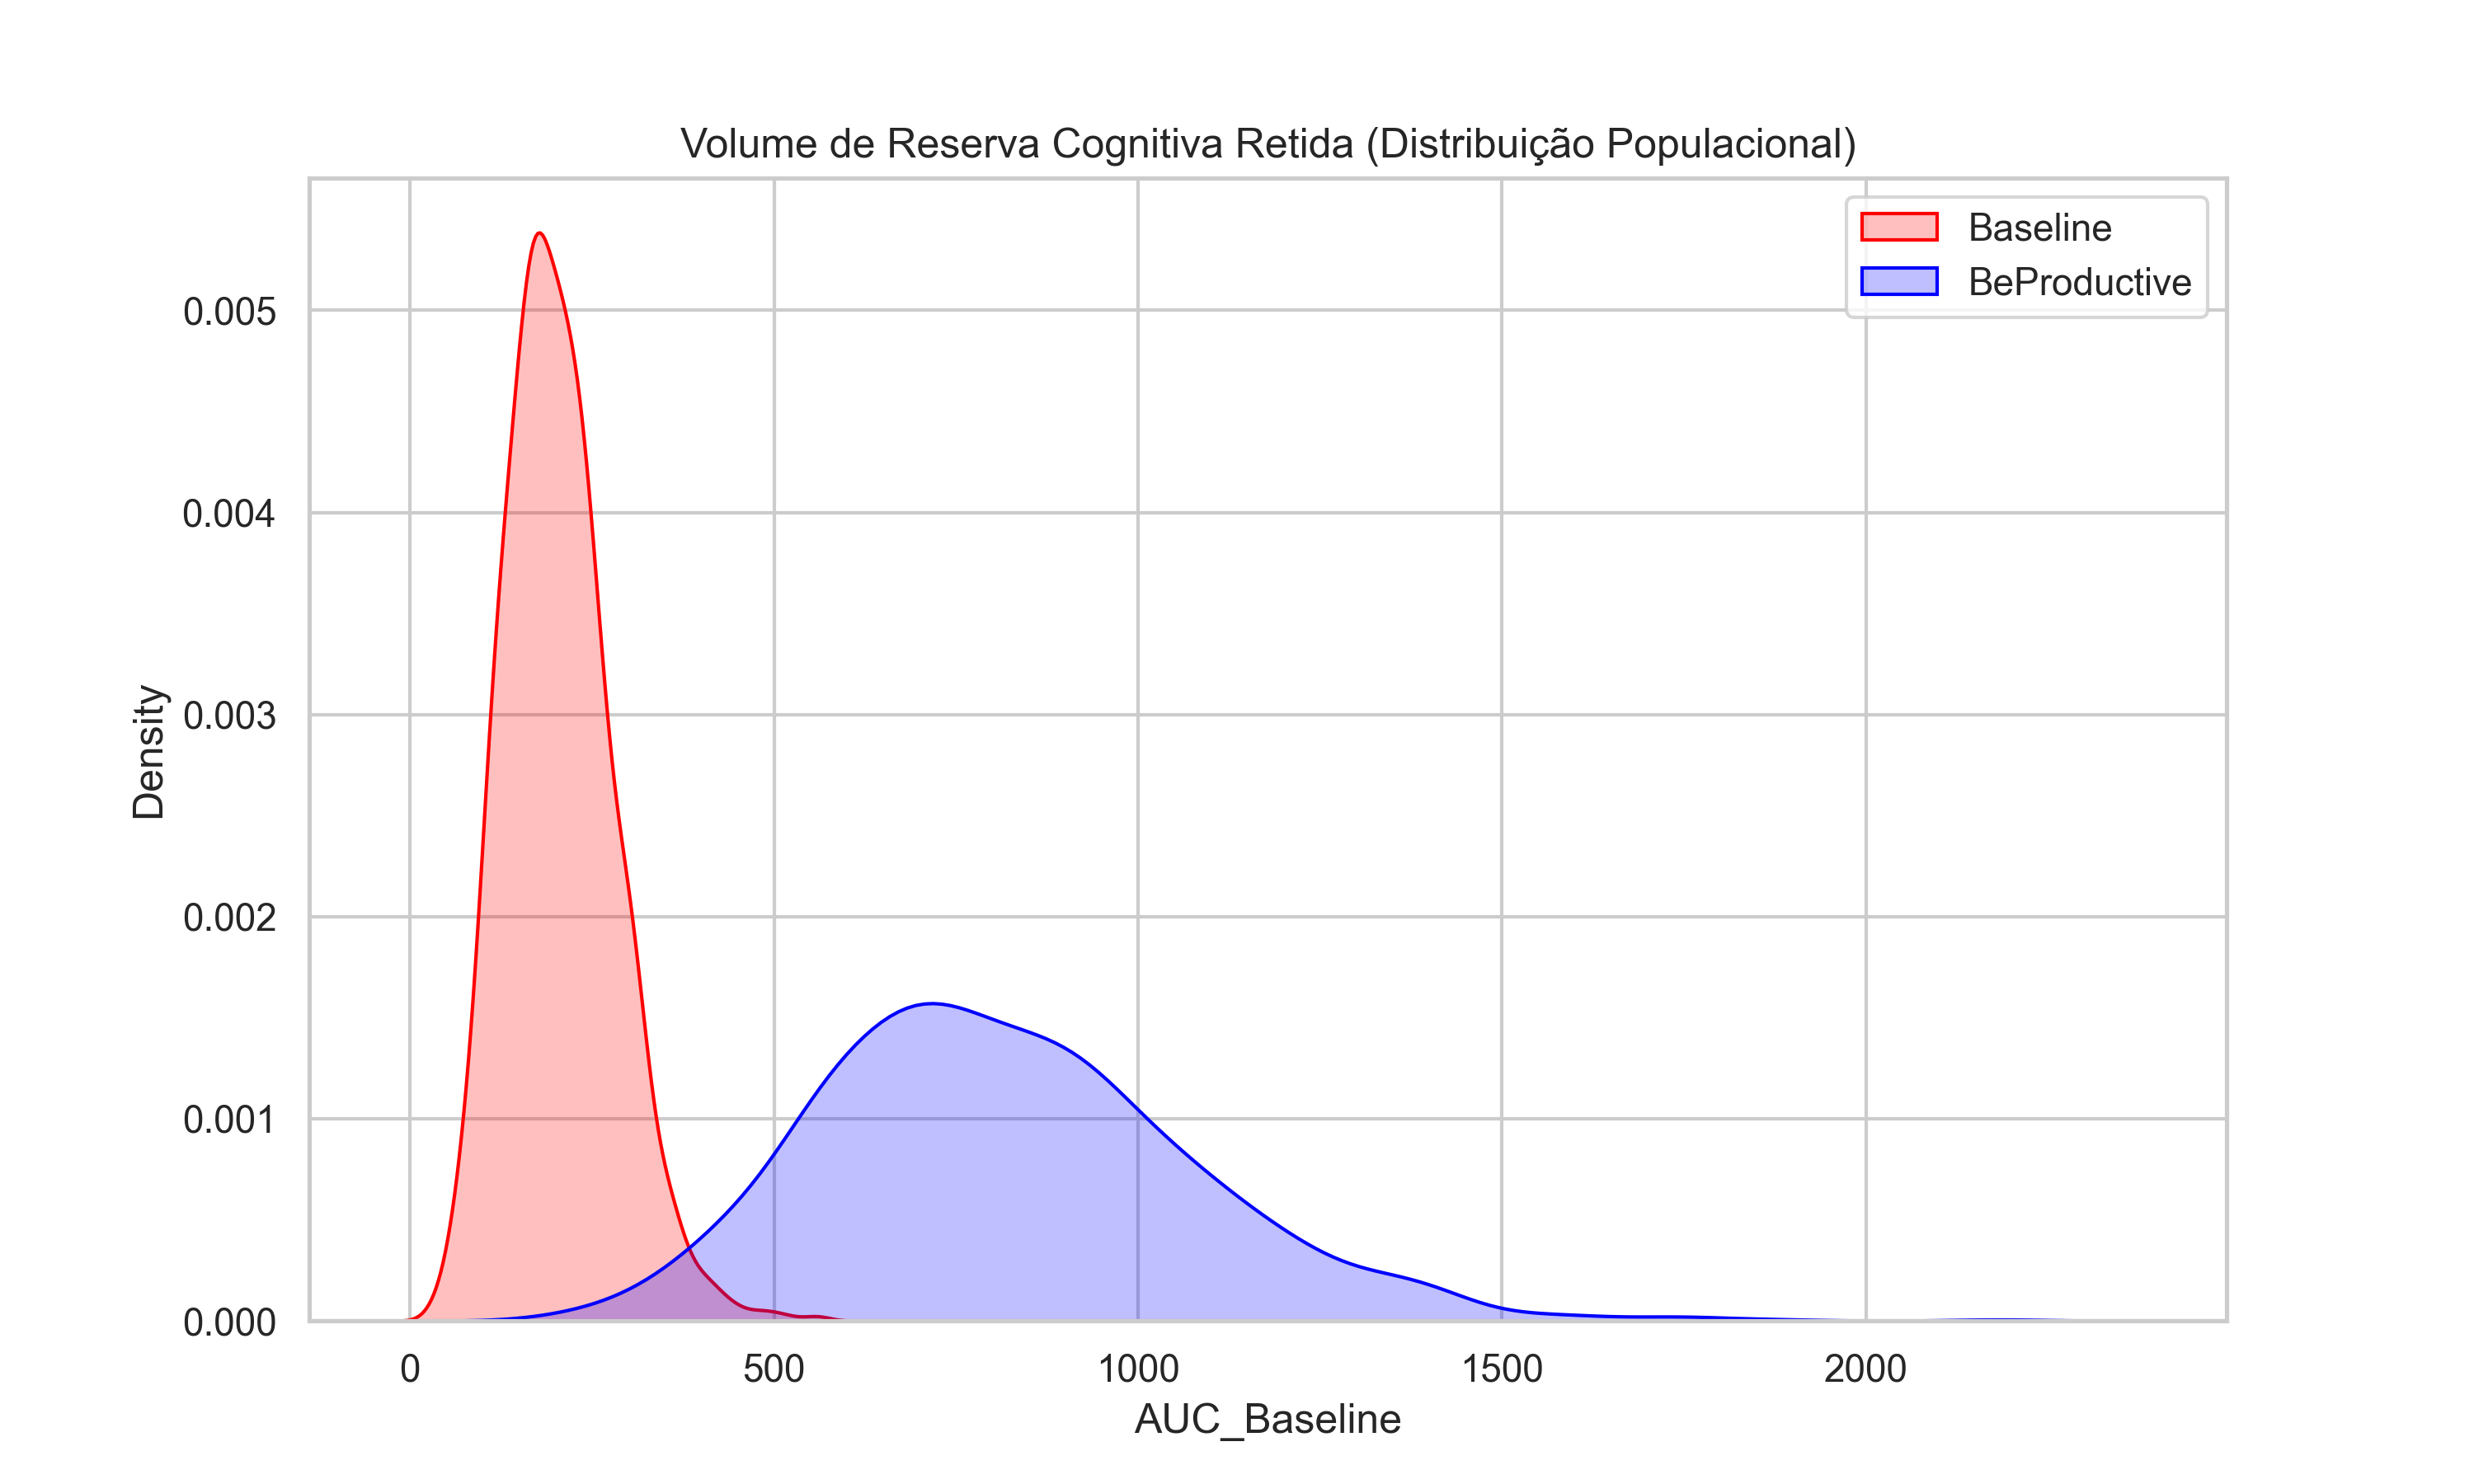
\includegraphics[width=0.8\textwidth]{../../fig_1_ego_depletion.png}
    \source{Elaborado pelos autores.}
    \label{fig:ego_depletion}
\end{figure}

\subsection{Alinhamento de Intenção e Consumo}

Utilizamos a Divergência de Kullback-Leibler ($D_{KL}$) para medir o desvio entre a intenção declarada do agente e a alocação de tempo real imposta pelo algoritmo. Como demonstrado na Figura \ref{fig:kl_divergence}, o modelo proposto reduziu drasticamente essa divergência, aproximando a mediana de zero. Isso prova que o sistema respeita a agência do usuário, mitigando o sequestro atencional típico das redes tradicionais.

\begin{figure}[H]
    \centering
    \caption{Análise de Divergência KL (Intenção vs. Alocação Real)}
    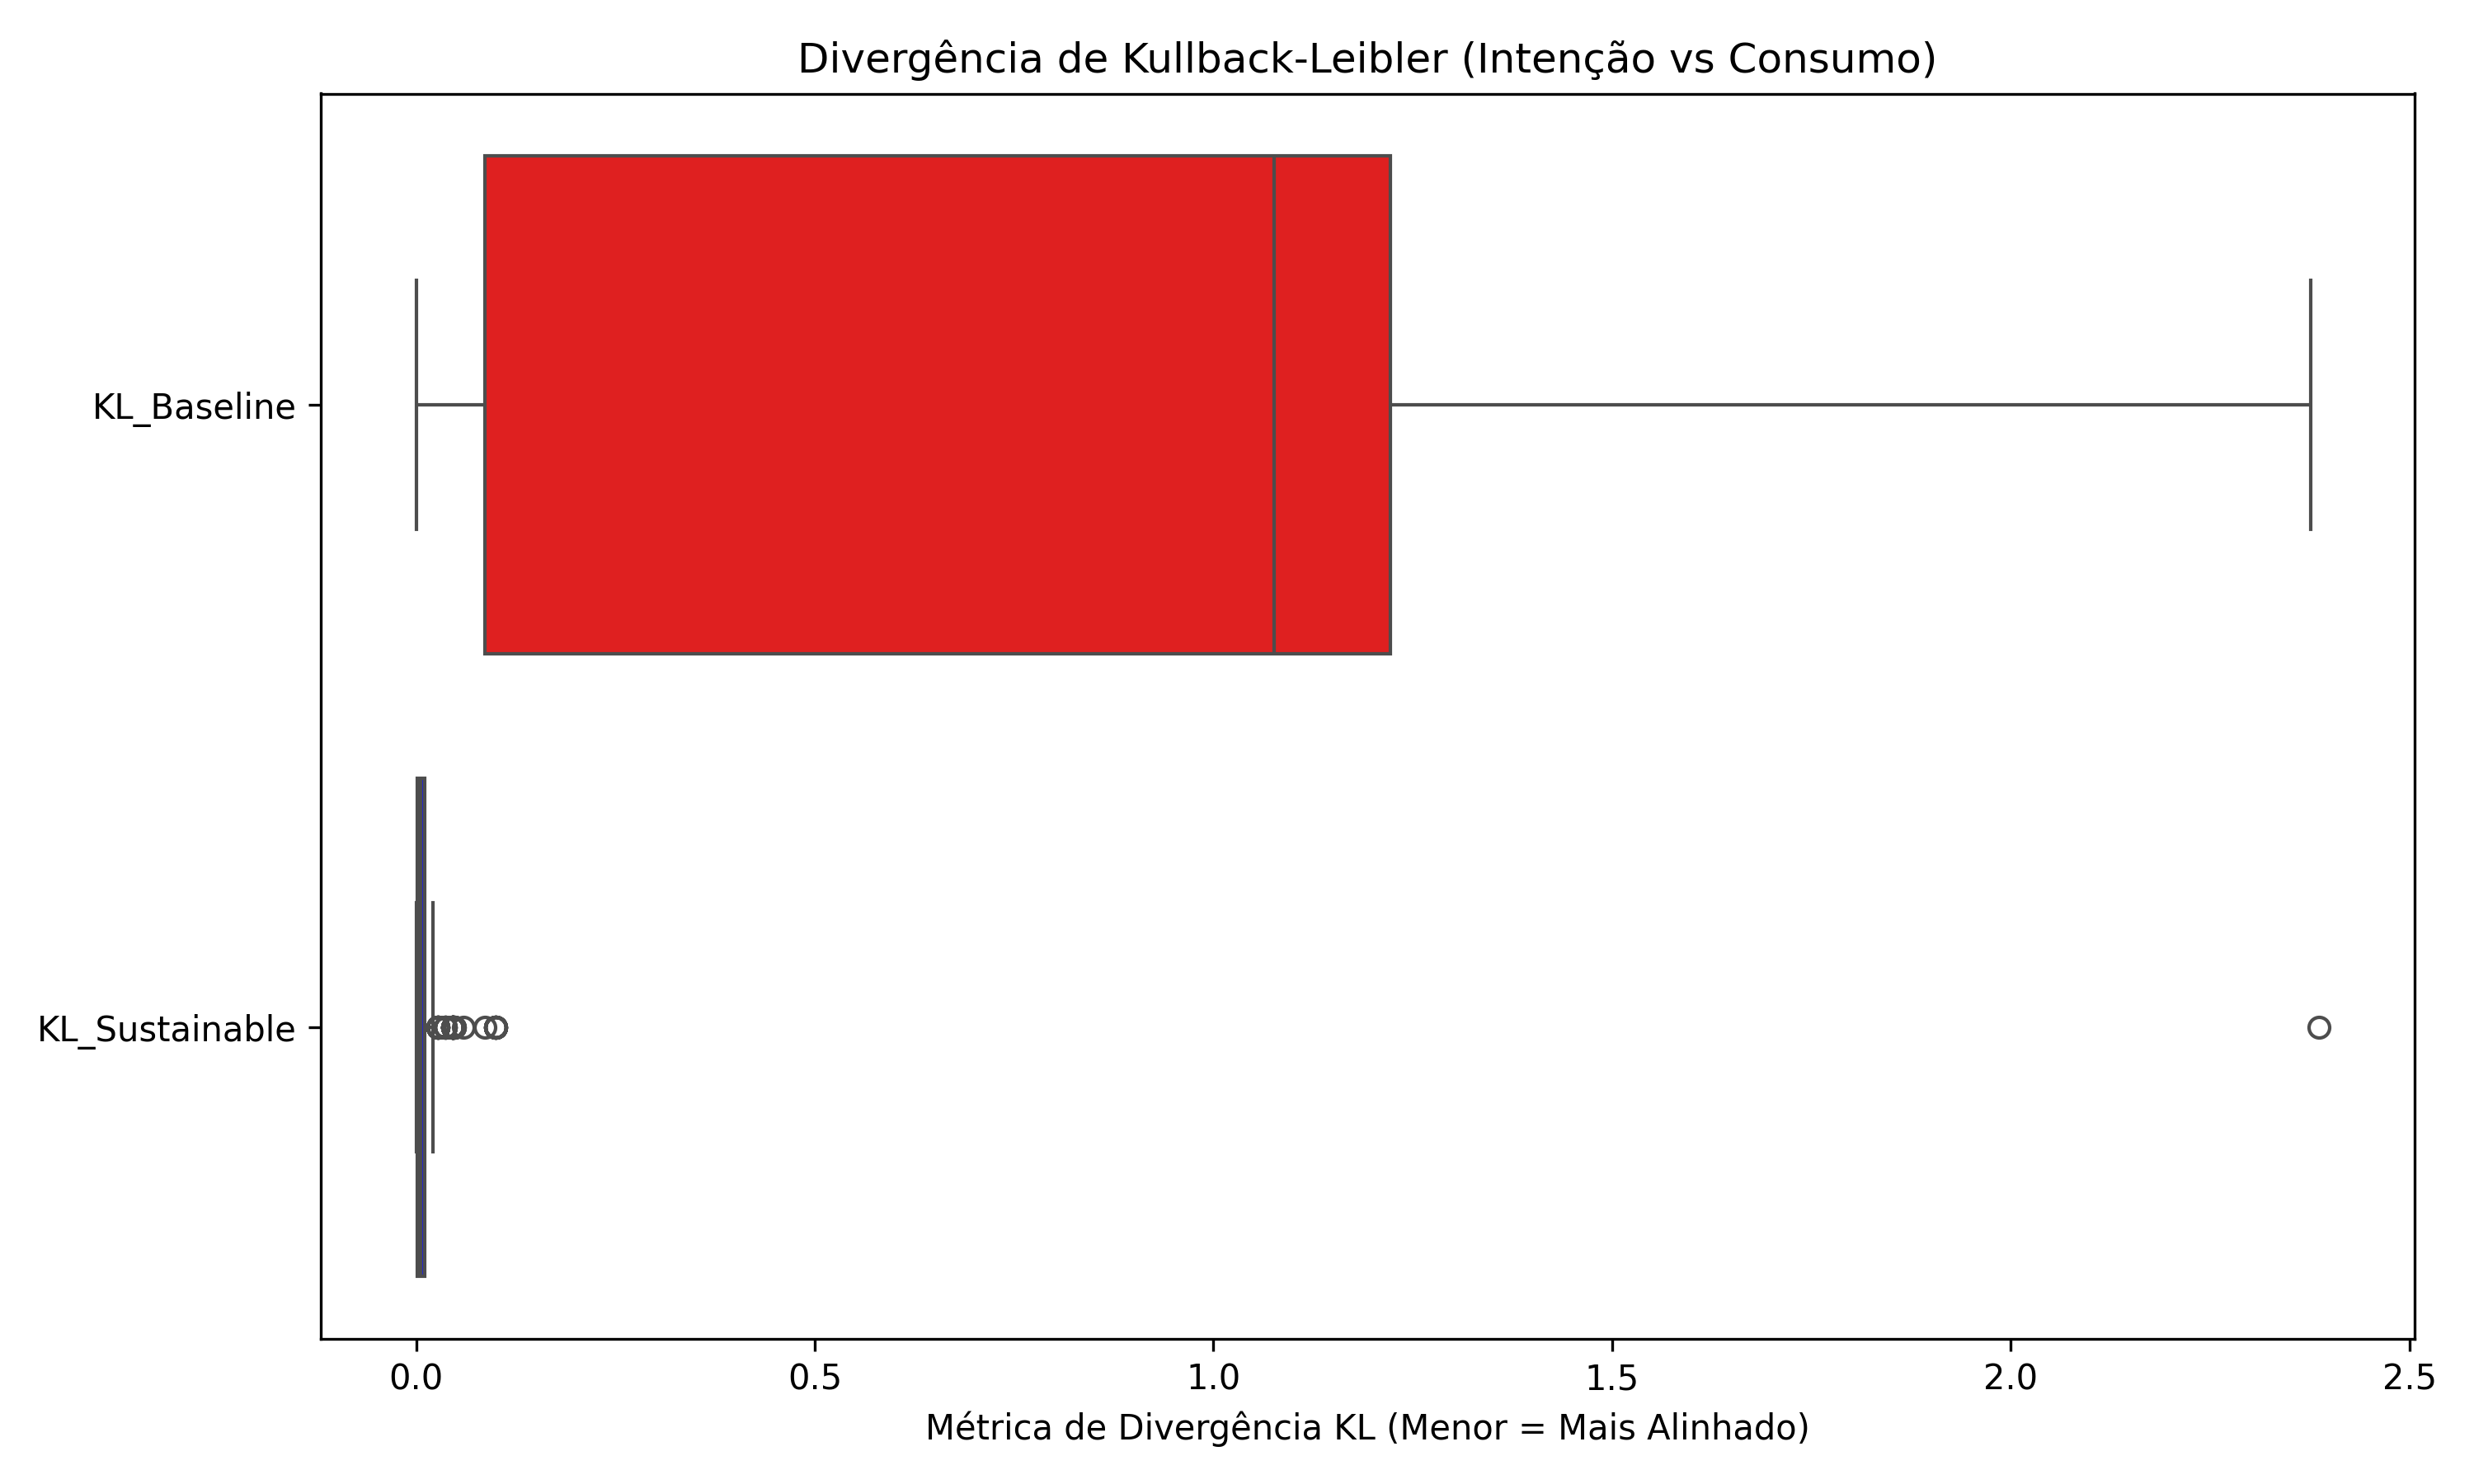
\includegraphics[width=0.8\textwidth]{../../fig_2_kl_divergence.png}
    \source{Elaborado pelos autores.}
    \label{fig:kl_divergence}
\end{figure}

\subsection{Robustez e Sensibilidade}

A robustez da solução foi testada via simulação de Monte Carlo. O mapa de calor na Figura \ref{fig:robustness} demonstra que o benefício algorítmico persiste em diversos cenários de fadiga e latência, comprovando que o modelo não é uma "solução de laboratório", mas uma arquitetura resiliente.

\begin{figure}[H]
    \centering
    \caption{Manifold de Robustez Atencional (Delta de AUC)}
    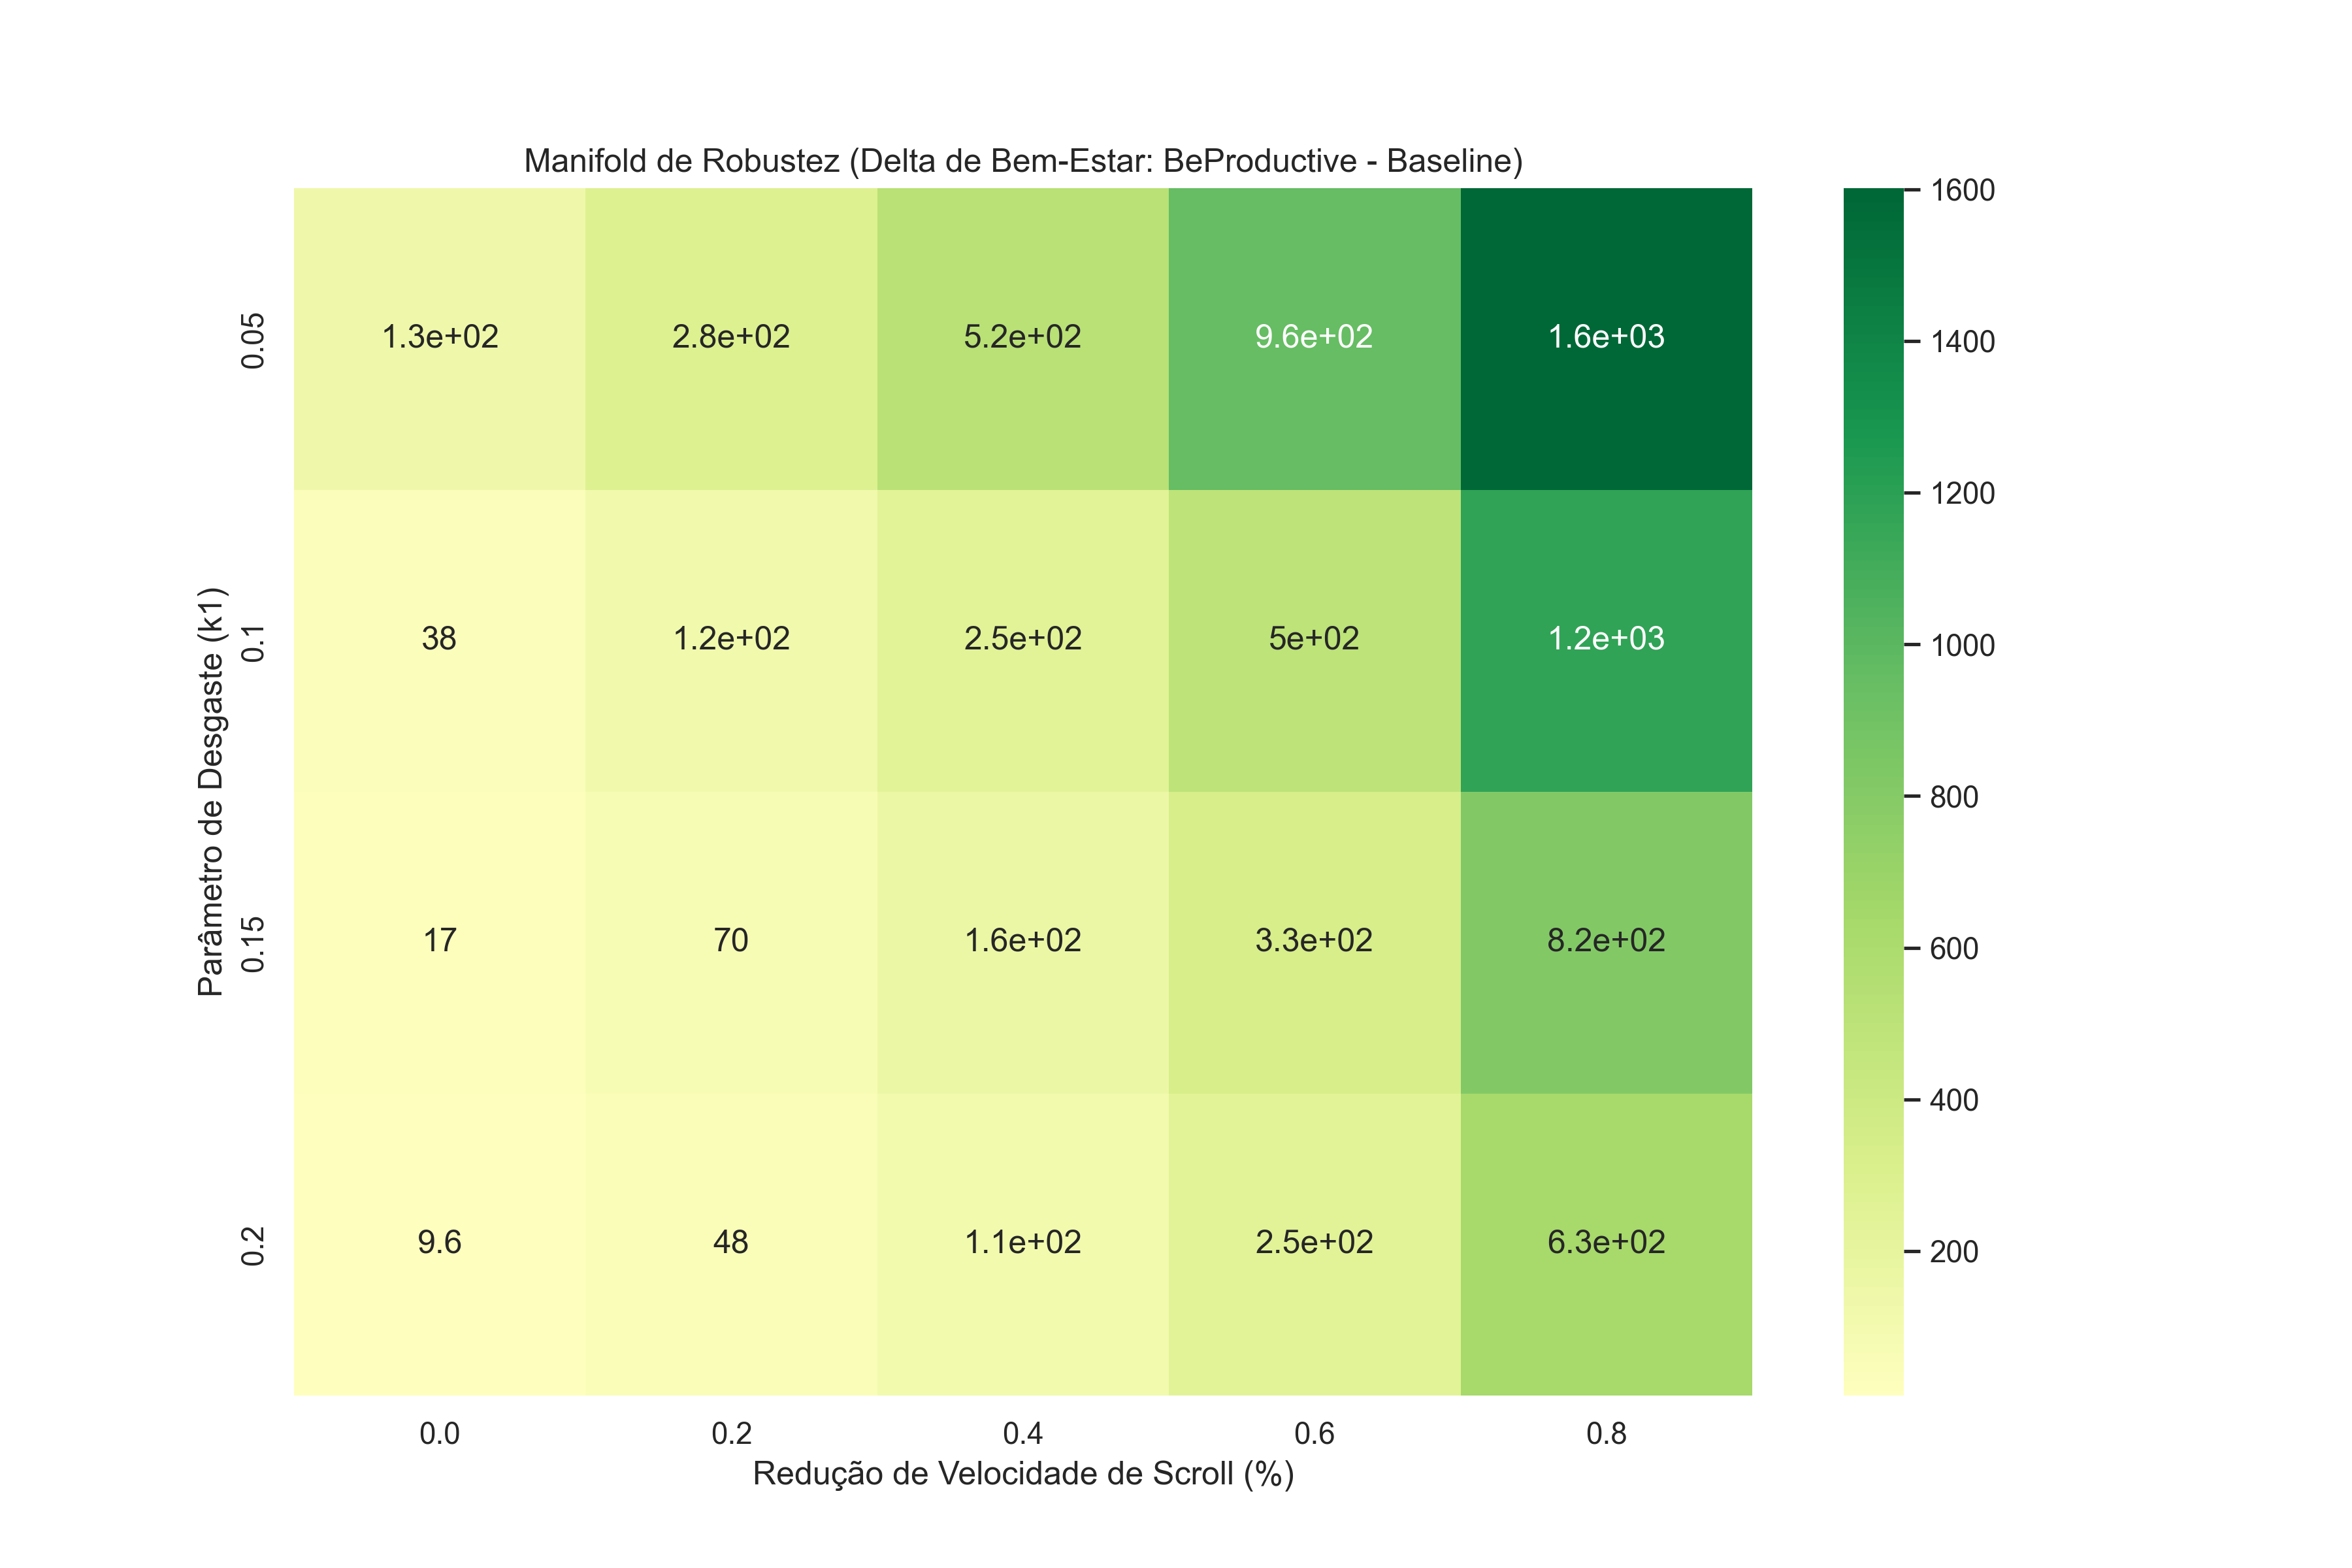
\includegraphics[width=0.8\textwidth]{../../fig_3_robustness_manifold.png}
    \source{Elaborado pelos autores.}
    \label{fig:robustness}
\end{figure}

\section{Implicações Éticas e Políticas Públicas}

A implementação do \textit{Be-Productive} via \textit{Edge AI} garante que métricas comportamentais sensíveis nunca deixem o dispositivo do usuário, estabelecendo um padrão de \textit{Privacy by Design}. Sob a ótica ética, a solução desloca o poder dos detentores de plataformas para o indivíduo, promovendo o que se denomina soberania atencional.

Sugere-se que tais arquiteturas sirvam de referência para futuras regulações de bem-estar digital, incentivando o desenvolvimento de tecnologias que atuem como extensões da cognição humana, e não como predadores dela.

\section{Conclusão}

Este trabalho consolidou a viabilidade técnica de uma arquitetura de recomendação voltada à atenção sustentável. Através da integração de Processos de Hawkes e dinâmica de sistemas, provamos ser possível otimizar a utilidade sem prescindir da integridade psicológica. O modelo \textit{Be-Productive} estabelece um novo paradigma para a Interação Humano-Computador, onde o alinhamento de valores deixa de ser um imperativo filosófico para tornar-se uma factibilidade de engenharia.

\section*{Referências}
\printbibliography[heading=none]

\newpage

\appendix
\section{Detalhamento Matemático dos Processos de Hawkes}

Nesta seção, apresentamos a formalização completa da intensidade condicional $\lambda(t)$ utilizada no modelo. Diferente do rascunho simplificado, a intensidade é decomposta em dois kernels exponenciais:
\begin{equation}
\lambda(t) = \mu + \sum_{t_k \in K, t_k < t} \alpha_1 e^{-\beta_1(t-t_k)} + \sum_{t_m \in M, t_m < t} \alpha_2 e^{-\beta_2(t-t_m)}
\end{equation}
Onde:
\begin{itemize}
    \item $\mu$: Taxa base de interação (propensão inata).
    \item $\alpha_1, \beta_1$: Magnitude e decaimento da excitação do Sistema 1 (impulsivo). No modelo calibrado, $\alpha_1 \gg \alpha_2$.
    \item $\alpha_2, \beta_2$: Magnitude e decaimento da excitação do Sistema 2 (deliberado). Aqui, $\beta_2 \to 0$, indicando persistência temporal do interesse.
\end{itemize}

O score de qualidade multiobjetivo ($Q$) que governa o ranqueamento é definido pela norma mínima dos classificadores de segurança multiplicada pelo componente de mérito:
\begin{equation}
Q(i, u) = \left[ \sum w_k f_k(i, u) \right] \times \min_m(1 - P_m(i))
\end{equation}
Essa formulação garante que conteúdos com alta probabilidade de toxicidade ou \textit{clickbait} ($P \approx 1$) tenham seu score efetivamente zerado.

\section{Parâmetros da Simulação Baseada em Agentes (ABM)}

Os agentes foram inicializados com as seguintes distribuições estocásticas para garantir realismo comportamental:
\begin{table}[H]
    \centering
    \caption{Parâmetros de Inicialização dos Agentes}
    \begin{tabular}{@{}lll@{}}
    \toprule
    Parâmetro & Distribuição & Descrição \\ \midrule
    $\mu$ & $Lognormal(0.5, 0.2)$ & Intensidade básica de uso \\
    $k$ & $Lognormal(-1.0, 0.5)$ & Taxa de desconto hiperbólico \\
    $R_{max}$ & $\mathcal{N}(100, 15)$ & Capacidade total da reserva \\
    $\kappa_1$ & Unif(0.05, 0.2) & Sensibilidade ao \textit{scroll} \\ \bottomrule
    \end{tabular}
    \source{Elaborado pelos autores.}
\end{table}

A integração numérica da EDO de reserva cognitiva foi realizada via método de Euler com passo $\Delta t = 0.1$. O código fonte modularizado e os registros de ensaios encontram-se sob versionamento para auditoria científica.

\end{document}
